\documentclass{beamer}
\usepackage[utf8]{inputenc}
\usepackage[UKenglish]{babel}
\usepackage[UKenglish]{isodate}
\usepackage{tikz}
\usepackage[style=authoryear,giveninits=true,uniquename=init]{biblatex}
\usepackage{complexity}
\usepackage[vlined]{algorithm2e}
\usepackage{spot}
\usepackage{appendixnumberbeamer}
\usepackage{csquotes}
\usepackage[clock]{ifsym}
\usepackage{amsmath}
\usepackage{mathtools}
\usepackage{siunitx}

\usetikzlibrary{arrows.meta}
\usetikzlibrary{tikzmark}
\usetikzlibrary{positioning}
\tikzstyle{every picture}+=[remember picture]
\tikzstyle{na} = [baseline=-.5ex]

\beamertemplatenavigationsymbolsempty
\usetheme{Madrid}
\usecolortheme{seahorse}
\addbibresource{talk.bib}
\DeclareMathOperator{\leftlsquigarrow}{\text{\reflectbox{$\rightsquigarrow$}}}
\DeclareMathOperator{\Vars}{Vars}

\definecolor{c1}{HTML}{1b9e77}
\definecolor{c2}{HTML}{d95f02}
\definecolor{c3}{HTML}{7570b3}
\definecolor{c4}{HTML}{e7298a}

\newcommand{\one}{\textcolor{c1}{x_1}}
\newcommand{\two}{\textcolor{c2}{x_2}}
\newcommand{\three}{\textcolor{c3}{x_3}}
\newcommand{\four}{\textcolor{c4}{x_4}}
\newcommand{\highlight}[1]{%
  \colorbox{red!10}{$#1$}}

\author{Paulius Dilkas}
\title{Generating Random WMC Instances}
\subtitle{An Empirical Analysis with Varying Primal Treewidth}
\institute[NUS]{National University of Singapore}
\date{30th May 2024}
% 40 min talk

\newif\iflattersubsect

\AtBeginSection[] {
    \begin{frame}<beamer>
    \frametitle{Overview} %
    \tableofcontents[currentsection]
    \end{frame}
    \lattersubsectfalse
}

\AtBeginSubsection[] {
    \iflattersubsect
    \begin{frame}<beamer>
    \frametitle{Overview} %
    \tableofcontents[currentsubsection]
    \end{frame}
    \fi
    \lattersubsecttrue
}

\begin{document}

\begin{frame}[noframenumbering,plain]
  \tikz[remember picture,overlay]{
    \node at ([yshift=20pt,xshift=-20pt]current page.south)
    {
\includegraphics[height=40pt]{nus.jpg}};
    \node at ([yshift=25pt,xshift=30pt]current page.south)
    {
\includegraphics[height=40pt]{inf.png}};
    \node at ([yshift=25pt,xshift=75pt]current page.south)
    {
\includegraphics[height=40pt]{ecr.jpg}};
    \node at ([yshift=20pt,xshift=140pt]current page.south)
    {
\includegraphics[height=20pt]{epsrc.png}};
  }
  \titlepage
\end{frame}

\section{Introduction}

\begin{frame}{Which Algorithm Is Better? It Depends on the Data}
  \begin{center}
    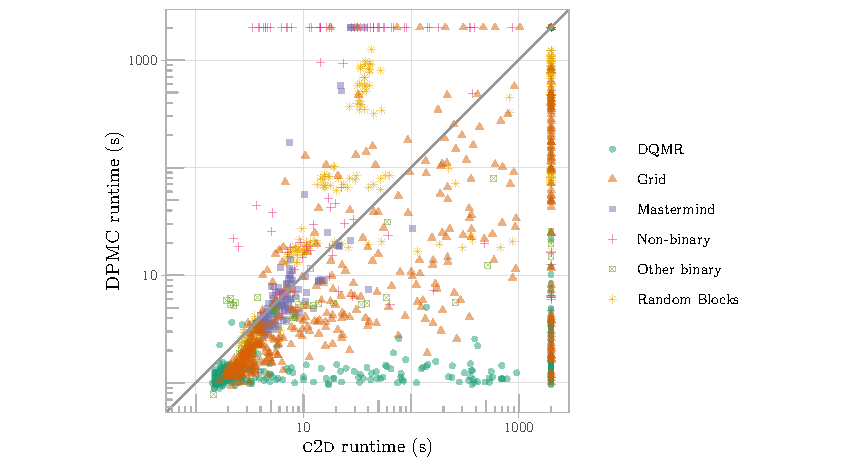
\includegraphics[width=\linewidth]{scatter}
  \end{center}

  The runtime data is from \textcolor{gray}{\textcite{DBLP:conf/sat/DilkasB21}}:
  various Bayesian networks encoded using the approach by
  \textcolor{gray}{\textcite{DBLP:conf/kr/Darwiche02}}
\end{frame}

\begin{frame}{The Problem: Weighted Model Counting (WMC)}
  \begin{columns}
    \begin{column}{0.5\textwidth}
      \begin{itemize}
        \item A generalisation of propositional model counting ($\#\SAT{}$)
        \item Applications:
        \begin{itemize}
          \item graphical models
          \item probabilistic programming
          \item neuro-symbolic AI
        \end{itemize}
        \item WMC algorithms use:
        \begin{itemize}
          \item dynamic programming
          \item knowledge compilation
          \item \SAT{} solvers
        \end{itemize}
      \end{itemize}
    \end{column}
    \begin{column}{0.5\textwidth}
      \begin{example}
        $w(x) = 0.3$, $w(\neg x) = 0.7$, $w(y) = 0.2$, $w(\neg y) = 0.8$
        \vspace{0.5cm}

        $\mathsf{WMC}(\alert{x \lor y}) = w(x)w(y) + w(x)w(\neg y) + w(\neg x)w(y) = 0.44$
      \end{example}
    \end{column}
  \end{columns}
\end{frame}

\begin{frame}{(Some of the) WMC Algorithms}
  \begin{itemize}
    \item \textsc{Cachet} \textcolor{gray}{\parencite{DBLP:conf/sat/SangBBKP04}}
          \begin{itemize}
            \item a SAT solver with \alert{clause learning} and \alert{component
                  caching}
          \end{itemize}
    \item \textsc{c2d} \textcolor{gray}{\parencite{DBLP:conf/ecai/Darwiche04}}
          \begin{itemize}
            \item knowledge compilation to \alert{d-DNNF}
          \end{itemize}
    \item \textsc{d4} \textcolor{gray}{\parencite{DBLP:conf/ijcai/LagniezM17}}
          \begin{itemize}
            \item knowledge compilation to \alert{decision-DNNF}
          \end{itemize}
    \item \textsc{miniC2D} \textcolor{gray}{\parencite{DBLP:conf/ijcai/OztokD15}}
          \begin{itemize}
            \item knowledge compilation to \alert{decision-SDDs}
          \end{itemize}
    \item \textsc{DPMC} \textcolor{gray}{\parencite{DBLP:conf/cp/DudekPV20}}
          \begin{itemize}
            \item dynamic programming with \alert{ADDs} and \alert{tree
                  decomposition} based planning
          \end{itemize}
  \end{itemize}
\end{frame}

\begin{frame}{Frequently Asked Questions}
  \begin{itemize}
    \item[Q:] \pause Why isn't \textsc{SharpSAT-TD} included in the experiments?
    \item[A:] Because I started setting up these experiments \alert{eight days}
          after the \textsc{SharpSAT-TD} paper came out
    \item[Q:] \pause Why isn't \textsc{GANAK} included in the experiments?
    \item[A:] Because it's easy to argue that probabilistic algorithms are
          \alert{out of scope} (and I had lots of algorithms already)
    \item[Q:] \pause Why am I giving a talk about this \alert{now}?
    \item[A:] 
\includegraphics[width=0.3\linewidth]{shrug}
  \end{itemize}
\end{frame}

\section{Background}

\begin{frame}{Knowledge Compilation: \alert<4>{d}-\alert<3>{D}\alert<2>{NNF} and
    \alert<5>{Decision}-\alert<3>{D}\alert<2>{NNF}}
  \begin{columns}
    \begin{column}{0.57\textwidth}
      \begin{description}
        \item<2->[Negation normal form:] \structure{$\neg$} is only applied to
              variables
        \item<3->[Decomposability:] for every \structure{$\alpha \land \beta$},
              \structure{$\Vars(\alpha) \cap \Vars(\beta) = \emptyset$}
        \item<4->[Determinism:] for every \structure{$\alpha \lor \beta$},
              \structure{$\alpha \land \beta \equiv \bot$}
        \item<5->[Decision:] all disjunctions are of the form

              \begin{tikzpicture}[level 1/.style={sibling distance=2cm}, level 2/.style={sibling distance=1cm}]
                \node[draw,circle] {$\lor$}
                child {node[draw,circle] {$\land$}
                  child {node[draw,rectangle] {$x$}}
                  child {node {$\vdots$}}
                }
                child {node[draw,circle] {$\land$}
                  child {node[draw,rectangle] {$\neg x$}}
                  child {node {$\vdots$}}
                }
                ;
              \end{tikzpicture}
      \end{description}
    \end{column}
    \begin{column}{0.43\textwidth}
      \begin{example}
        \structure{$C \land (A \lor \neg B)$} in d-DNNF/decision-DNNF:
      \begin{center}
      \begin{tikzpicture}[level distance=0.8cm]
        \node[draw,circle] {$\land$}
        child {node[draw,circle] {$\lor$}
          child {node[draw,circle] (parent) {$\land$}
            child {node[draw,rectangle] {$B$}}
            child {edge from parent[draw=none]}
          }
          child {node[draw,circle] {$\land$}
            child {node[draw,circle] {$\lor$}
              child {node[draw,rectangle] (A) {$A$}}
              child {node[draw,rectangle] {$\neg A$}}
            }
            child {node[draw,rectangle] {$\neg B$}}
          }
        }
        child {node[draw,rectangle] {$C$}};
        \draw (parent) -- (A);
      \end{tikzpicture}
      \end{center}
      \end{example}
    \end{column}
  \end{columns}
\end{frame}

\begin{frame}[t]{Tree Decompositions and Primal Treewidth}
  A formula in CNF:
  \[
    \phi = \begin{aligned}(x_1 \lor x_2) \land (x_2 \lor x_3 \lor x_4) \land (x_1 \lor x_4) &\land (x_3 \lor x_5) \land (x_4 \lor x_5 \lor x_6) \\ &\land (x_5 \lor x_6 \lor x_7) \land (x_6 \lor x_7)\end{aligned}
  \]
  \pause
  \begin{columns}[t]
    \begin{column}{0.49\textwidth}
      The primal graph of \structure{$\phi$} is:
      \begin{center}
        \begin{tikzpicture}
          \node (x1) at (0, 0) {$x_1$};
          \node (x2) at (1, 1) {$x_2$};
          \node (x3) at (2, 1) {$x_3$};
          \node (x4) at (1, 0) {$x_4$};
          \node (x5) at (2, 0) {$x_5$};
          \node (x6) at (3, 0) {$x_6$};
          \node (x7) at (4, 0) {$x_7$};
          \draw (x1) -- (x2);
          \draw (x1) -- (x4);

          \draw (x2) -- (x3);
          \draw (x2) -- (x4);

          \draw (x3) -- (x4);
          \draw (x3) -- (x5);

          \draw (x4) -- (x5);
          \draw (x4) to[bend right] (x6);

          \draw (x5) -- (x6);
          \draw (x5) to[bend left] (x7);

          \draw (x6) -- (x7);
        \end{tikzpicture}

        \vspace{1.5cm}
        \onslide<4>{$\therefore$ the primal treewidth of \structure{$\phi$} is \structure{2}}
      \end{center}
    \end{column}%
    \begin{column}{0.49\textwidth}
      \pause
      Its minimum-width tree decomposition:
      \begin{center}
        \begin{tikzpicture}[sibling distance=5em]
          \node {$\{x_4, x_5, x_6\}$}
          child { node {$\{x_1, x_4\}$}
            child { node {$\{x_1, x_2\}$} }
          }
          child { node {$\{x_2, x_3, x_4\}$}
            child { node {$\{x_3, x_5\}$} }
          }
          child { node {$\{x_5, x_6, x_7\}$}
            child { node {$\{x_6, x_7\}$} }
          };
        \end{tikzpicture}
      \end{center}
    \end{column}
  \end{columns}
\end{frame}

\begin{frame}{Formally\dots}
\begin{definition}[\cite{DBLP:journals/jct/RobertsonS84}]\label{def:treewidth}
  A \alert{tree decomposition} of a graph \structure{$G$} is a pair
  \structure{$(T, \chi)$}, where \structure{$T$} is a tree and
  \structure{$\chi\colon \mathcal{V}(T) \to 2^{\mathcal{V}(G)}$} is a labelling
  function, with the following properties:
  \begin{itemize}
    \item \structure{$\bigcup_{t \in \mathcal{V}(T)} \chi(t) = \mathcal{V}(G)$};
    \item for every edge \structure{$e \in \mathcal{E}(G)$}, there is
          \structure{$t \in \mathcal{V}(T)$} s.t.\ \structure{$e$} has both
          endpoints in \structure{$\chi(t)$};
    \item for all \structure{$t, t', t'' \in \mathcal{V}(T)$}, if
          \structure{$t'$} is on the path between \structure{$t$} and
          \structure{$t''$}, then
          \structure{$\chi(t) \cap \chi(t'') \subseteq \chi(t')$}.
  \end{itemize}
  The \alert{width} of tree decomposition \structure{$(T, \chi)$} is
  \structure{$\max_{t \in \mathcal{V}(T)} |\chi(t)| - 1$}. The \alert{treewidth}
  of graph \structure{$G$} is the smallest \structure{$w$} such that
  \structure{$G$} has a tree decomposition of width \structure{$w$}.
\end{definition}
\end{frame}

\begin{frame}{The Parameterised Complexity of WMC Algorithms}
  Let \structure{$n$} be the number of \alert{variables} and \structure{$m$} be
  the number of \alert{clauses}.
  \begin{itemize}
    \item Component caching (used in \textsc{Cachet}) is
          \structure{$2^{\mathcal{O}(w)}n^{\mathcal{O}(1)}$}, where
          \structure{$w$} is the \alert{branchwidth} of the underlying
          hypergraph
          \textcolor{gray}{\parencite{DBLP:journals/jair/BacchusDP09}}
          \begin{itemize}
            \item Branchwidth is within a constant factor of primal treewidth
          \end{itemize}
    \item \textsc{c2d} is based on an algorithm, which is
          \structure{$\mathcal{O}(2^{w}mw)$}, where \structure{$w$} is at most
          \alert{primal treewidth}
          \textcolor{gray}{\parencite{DBLP:journals/jacm/Darwiche01,DBLP:conf/ecai/Darwiche04}}
    \item \textsc{DPMC} can be shown to be \structure{$\mathcal{O}(4^{w}mn)$},
          where \structure{$w$} is an upper bound on \alert{primal treewidth}
  \end{itemize}
\end{frame}
% NOTE: could add a slide that outlines the proof of DPMC's parameterised
% complexity (I have the full proof in my notes)

\begin{frame}{Early History of Random SAT}
  \begin{itemize}
    \item \textcolor{gray}{\textcite{DBLP:journals/ipl/GoldbergPB82}} show that
          (simplified) \alert{Davis-Putnam procedures} run in \alert{polynomial
          time} on average on the following model:
          \begin{itemize}
            \item Fix the numbers of \alert{variables} and \alert{clauses}
            \item Let \structure{$p \in (0, 0.5)$}
            \item For each clause \structure{$C$} and variable \structure{$x$}:
            \begin{itemize}
              \item \alert{Add} \structure{$x$} to \structure{$C$} w.p.\
                    \structure{$p$}
              \item Or \alert{add} \structure{$\neg x$} to \structure{$C$} w.p.\
                    \structure{$p$}
              \item Or \alert{do nothing} w.p.\ \structure{$1 - 2p$}
            \end{itemize}
          \end{itemize}
          \pause
    \item \textcolor{gray}{\textcite{DBLP:journals/dam/FrancoP83}} were the
          first to propose a `reasonable' random \structure{$k$}-CNF model:
    \begin{enumerate}
      \item Fix the numbers of \alert{variables}, \alert{clauses}, and
            \alert{clause width}
      \item \alert{Sample each clause} independently as a subset of all possible
            literals
      \item \alert{Reject} clauses that have \structure{$x$} and
            \structure{$\neg x$} for some variable \structure{$x$}
    \end{enumerate}
    \begin{itemize}
      \item They show that the Davis-Putnam procedure \alert{requires
            exponential time} w.p.\ \structure{$1$}
    \end{itemize}
  \end{itemize}
\end{frame}

\begin{frame}{Phase Transitions}
  \begin{itemize}
    \item Phase transitions for \alert{decision problems} have been studied both
          \alert{experimentally} and \alert{theoretically} for a long time (see,
          e.g.,
          \textcolor{gray}{\textcite{DBLP:conf/ijcai/CheesemanKT91}})\pause
    \item Phase transitions are characterised by a parameter \structure{$k$}
          such that:
    \begin{itemize}
      \item For \alert{low} values of \structure{$k$}, the problem is
            \alert{easy}
      \item For \alert{high} values of \structure{$k$}, the problem is
            \alert{easy} again
      \item \alert{Average} values of \structure{$k$} is where the problem
            becomes \alert{hard}\pause
    \end{itemize}
    \item For SAT-based problems, \alert{(clause) density} is the standard
          parameter
          \begin{itemize}
            \item i.e., the number of \alert{clauses} divided by the number of
                  \alert{variables}
            \item (usually parameterised by \alert{clause width})\pause
          \end{itemize}
    \item The most comprehensive (experimental) study of phase transitions for
          \alert{SAT algorithms} is
          by~\textcolor{gray}{\textcite{DBLP:journals/constraints/CoarfaDASV03}}
          \begin{itemize}
            \item They show that the transition from polynomial to exponential
                  time \alert{depends on the solver}
          \end{itemize}
  \end{itemize}
\end{frame}
% NOTE: I could add a lot more of this

\section{Random WMC}

\begin{frame}{Generating Random WMC Instances: The Algorithm}
  \begin{columns}
    \begin{column}{0.69\textwidth}
      \begin{algorithm}[H]
        \SetKwData{kcnf}{kcnf}
        \SetKwFunction{NewVariable}{newVariable}
        $\structure{\phi} \gets \text{empty CNF formula}$\;
        $\structure{G} \gets \text{empty graph}$\;
        \For{$i \gets 1$ \KwTo \alert{$m$\tikz[na] \node[coordinate] (m1) {};}}{
          $\structure{X} \gets \emptyset$\;
          \For{$j \gets 1$ \KwTo \alert{$k$\tikz[na] \node[coordinate] (k1) {};}}{
            $\structure{x} \gets \alert{\NewVariable{$X$, $G$}}\tikz[na] \node[coordinate] (f1) {};$\;
            $\mathcal{V}(\structure{G}) \gets \mathcal{V}(\structure{G}) \cup \{\, \structure{x} \,\}$\;
            $\mathcal{E}(\structure{G}) \gets \mathcal{E}(\structure{G}) \cup \{\, \{\,\structure{x}, \structure{y}\,\} \mid \structure{y} \in \structure{X} \,\}$\;
            $\structure{X} \gets \structure{X} \cup \{\, \structure{x} \,\}$\;
          }
          $\structure{\phi} \gets \structure{\phi} \cup \{\,\{\, \structure{l} \leftlsquigarrow \mathcal{U}\{\, \structure{x}, \neg \structure{x} \,\} \mid \structure{x} \in \structure{X} \,\}\,\}$\tikz[na] \node[coordinate] (c1) {};\;
        }
      \end{algorithm}
    \end{column}
    \begin{column}{0.31\textwidth}
      \begin{itemize}
        \item\tikz[na] \node[coordinate] (m2) {};the number of clauses
        \item\tikz[na] \node[coordinate] (k2) {};clause width
        \item\tikz[na] \node[coordinate] (f2) {};a function to pick a variable
        \item\tikz[na] \node[coordinate] (c2) {};a (fair) coin flip
      \end{itemize}
    \end{column}
  \end{columns}
  \begin{tikzpicture}[overlay]
    \path[-Latex,shorten >=0.6cm,shorten <=0.5cm,dashed] (m2) edge (m1);
    \path[-Latex,shorten >=0.6cm,shorten <=0.5cm,dashed] (k2) edge (k1);
    \path[-Latex,shorten >=0.1cm,shorten <=0.5cm,dashed] (f2) edge (f1);
    \path[-Latex,shorten >=0.1cm,shorten <=0.5cm,dashed] ([shift={(0, 0.2)}]c2) edge (c1);
  \end{tikzpicture}
\end{frame}

\begin{frame}{How to Pick a Variable}
  Parameter \structure{$\rho \in [0, 1]$} biases the probability distribution
  towards adding variables that would introduce fewer new edges.

  \begin{algorithm}[H]
    \SetKwProg{Fn}{Function}{:}{}
    \Fn{\NewVariable{set of variables \structure{$X$}, primal graph \structure{$G$}}}{
      $\structure{N} \gets \{\, \structure{e} \in \mathcal{E}(\structure{G}) \mid |\structure{e} \cap \structure{X}| = 1 \,\}$\;
      \lIf{$\structure{N} = \emptyset$}{\Return{$\structure{x} \leftlsquigarrow \mathcal{U}(\{\, \structure{x_1}, \structure{x_2}, \dots, \structure{x_{\alert{n}}} \,\} \setminus \structure{X})$}}
      \Return{$\structure{x} \leftlsquigarrow \left(\{\, \structure{x_1}, \structure{x_2}, \dots, \structure{x}_{\alert{n}} \,\} \setminus \structure{X}, \structure{y} \mapsto \highlight{\frac{1 - \alert{\rho}}{\alert{n} - |\structure{X}|} + \alert{\rho}\frac{|\{\, \structure{z} \in X \mid \{\,\structure{y}, \structure{z}\,\} \in \mathcal{E}(\structure{G}) \,\}|}{|\structure{N}|}}\right)$}\;
    }
  \end{algorithm}
\end{frame}

\begin{frame}{From Random SAT to Random WMC}
  We introduce parameter \structure{$\rho \in [0, 1]$} that biases the
  probability distribution towards adding variables that would introduce fewer
  new edges to the primal graph.

  \vfill
  \begin{columns}[t]
    \begin{column}{0.5\linewidth}
      Example partially-filled formula:
      \structure{$(\neg x_{5} \lor x_{2} \lor x_{1}) \land (x_{5} \lor \alert{\mathord{?}} \lor \mathord{?})$}
    \end{column}
    \begin{column}{0.4\linewidth}
      Its primal graph:

      \begin{tikzpicture}
        \node (a) at (0.5, 1) {$x_{1}$};
        \node (b) at (0, 0) {$x_{2}$};
        \node (c) at (1, 0) {\spot{$x_{5}$}};
        \node (d) at (2, 1) {$x_{3}$};
        \node (e) at (2, 0) {$x_{4}$};
        \draw (a) -- (b);
        \draw[blue,thick] (b) -- (c);
        \draw[blue,thick] (c) -- (a);
        \draw (current bounding box.north east) rectangle (current bounding box.south west);
      \end{tikzpicture}
    \end{column}
  \end{columns}

  \begin{block}{The probability distribution for the next variable}
    Base probability of each variable being chosen:
    \[
      \frac{1 - \rho}{4}.
    \]

    Both \structure{$x_{1}$} and \structure{$x_{2}$} get a bonus probability of
    \structure{$\rho/2$} for each being the endpoint of \alert{one} out of
    the \alert{two} neighbourhood edges.
  \end{block}
\end{frame}

\section{Experiments}

\subsection{Validation}

\begin{frame}{The Relationship Between \structure{$\rho$} and Primal Treewidth}
  \begin{block}{Experiment 1 (Validation)}
    \begin{itemize}
      \item Set the number of variables to \structure{$100$}
      \item Consider a geometric sequence of \structure{$11$} densities from
            \structure{$0.4$} to \structure{$14.1$}
      \item Let \structure{$\rho$} range from \structure{zero} to
            \structure{one} in steps of \structure{$0.01$}
      \item Generate \structure{ten} \structure{$2$}-, \structure{$3$}-,
            \structure{$4$}-, and \structure{$5$}-CNF formulas
    \end{itemize}
  \end{block}
\end{frame}

\begin{frame}{The Relationship Between \structure{$\rho$} and Primal Treewidth}
  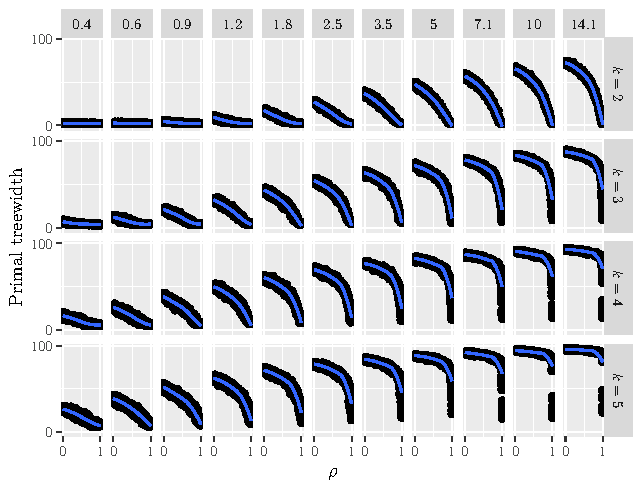
\includegraphics{regular_repetitiveness.pdf}
\end{frame}

\subsection{Hardness}

\begin{frame}{Density, Primal Treewidth, and Runtime}
  \begin{block}{Experiment 2 (The Main One)}
    \begin{itemize}
      \item Set the number of variables to \structure{$70$}
      \item Consider densities ranging from \structure{$1$} to \structure{$4.3$}
            in steps of \structure{$0.3$}
      \item Let \structure{$\rho$} range from \structure{$0$} to
            \structure{$0.5$} in steps of \structure{$0.01$}
      \item Generate one \structure{$3$}-CNF formula
    \end{itemize}
  \end{block}
\end{frame}

\begin{frame}{Peak Hardness w.r.t. Density}
  Let \structure{$\mu$} denote the \alert{density}, i.e., the number of clauses
  divided by the number of variables.
  \begin{itemize}
    \item \textsc{Cachet} is known to peak at \structure{$\mu = 1.8$}
          \textcolor{gray}{\parencite{DBLP:conf/sat/SangBBKP04}}
    \item \textcolor{gray}{\textcite{DBLP:conf/aaai/Pehoushek00}} show some
          $\#\SAT{}$ algorithms to peak at \structure{$\mu = 1.2$} and
          \structure{$\mu = 1.9$}
          \pause
    \item In our experiments:
    \begin{itemize}
      \item \textsc{DPMC} peaks at \structure{$\mu = 2.2$}
      \item all other algorithms peak at \structure{$\mu = 1.9$}
    \end{itemize}
  \end{itemize}
\end{frame}

\begin{frame}{Peak Hardness w.r.t. Density (when $\rho = 0$)}
  \centering
  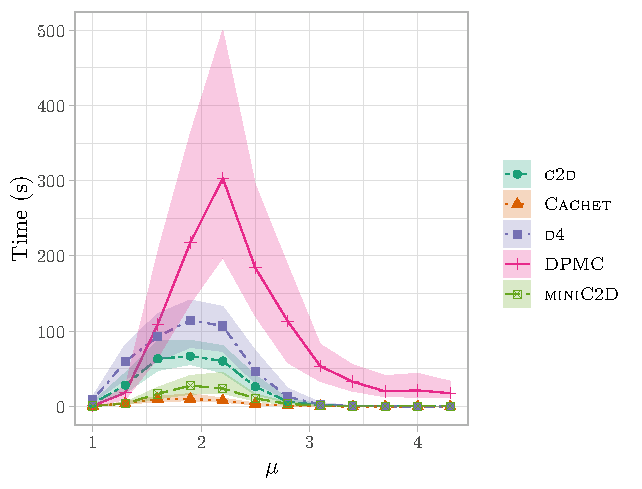
\includegraphics{treewidth.pdf}
\end{frame}

\begin{frame}{Hardness w.r.t. Primal Treewidth (when $\mu = 1.9$)}
  \centering
  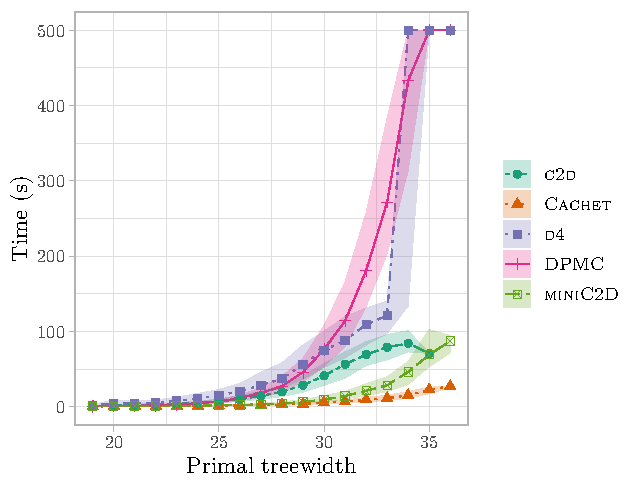
\includegraphics{treewidth2.pdf}
\end{frame}

\subsection{Statistical Analysis}

\begin{frame}{Is The Relationship Exponential: Two Approaches}
  \begin{block}{Linear Regression}
    We fit the model \structure{$\ln t \sim \alpha w + \beta$}, i.e.,
    \structure{$t \sim e^{\beta}{(e^{\alpha})}^{w}$}, where \structure{$t$} is
    \alert{runtime}, and \structure{$w$} is \alert{primal treewidth}
    \end{block}
    \begin{block}{Empirical Scaling Analyzer (ESA)
        v2~\parencite{DBLP:conf/gecco/PushakH20}}
    \begin{enumerate}
      \item Prepare a list of hypotheses about scalability, e.g.:
      \begin{description}
        \item[exponential:] \structure{$t \sim \alpha \beta^{w}$},
        \item[polynomial:] \structure{$t \sim \alpha w^{\beta}$}
      \end{description}
      \item Use \structure{\SI{30}{\percent}} of the data with the largest
            values of \structure{$w$} for testing
      \item For each hypothesis, ESA produces:
      \begin{itemize}
        \item estimates of parameter values,
        \item support loss, and
        \item challenge loss
      \end{itemize}
    \end{enumerate}
  \end{block}
\end{frame}
% NOTE: could show some of the tables/plots produced by ESA

\begin{frame}{How Well Does Linear Regression Explain the Data?}
  \centering
  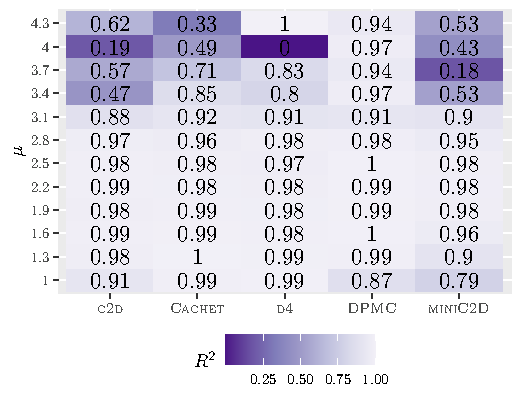
\includegraphics{r2.pdf}
\end{frame}

\begin{frame}{The Base of the Exponential}
  \centering
  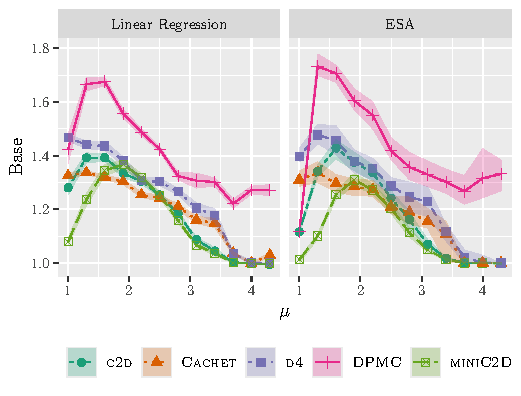
\includegraphics{linearbase2.pdf}
\end{frame}

\subsection{Miscellaneous}

\begin{frame}{Does Real Data Confirm Our Observations?}
  \centering
  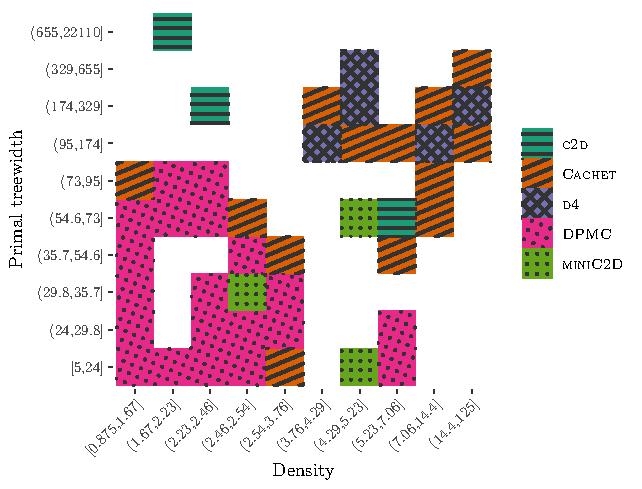
\includegraphics{real}
\end{frame}

\begin{frame}{Bonus 1: How \textsc{DPMC} Reacts to Redundancy in Weights}
  \centering
  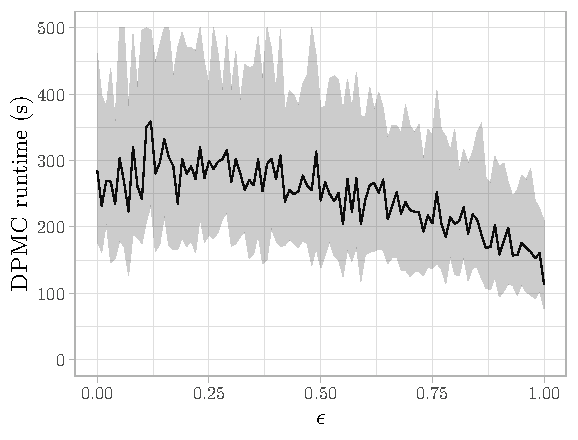
\includegraphics{epsilon}
\end{frame}

\begin{frame}{Bonus 2: 0/1 Weights Make Counting Easy}
  \centering
  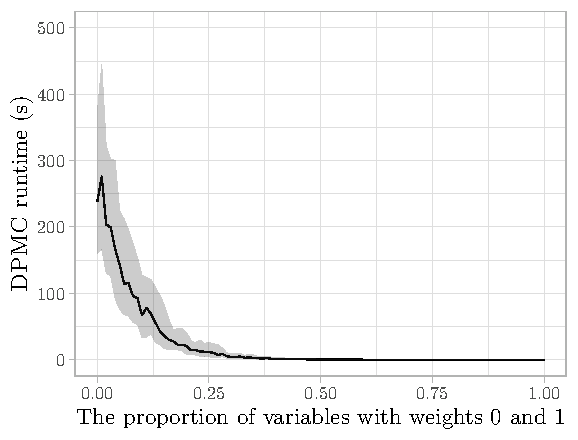
\includegraphics{delta}
\end{frame}

\section{Conclusion}

\begin{frame}{Summary}
  \begin{itemize}
    \item This work introduced a \alert{random model} for WMC instances with a
          parameter that indirectly controls \alert{primal treewidth}
    \item Observations:
    \begin{itemize}
      \item All algorithms \alert{scale exponentially} w.r.t.\ primal treewidth
      \item The running time of \textsc{DPMC}:
      \begin{itemize}
        \item peaks at a higher density
        \item and scales worse w.r.t.\ primal treewidth
      \end{itemize}
    \end{itemize}
    \item Future work:
    \begin{itemize}
      \item A theoretical relationship between \structure{$\rho$} and primal treewidth
      \item Non-\structure{$k$}-CNF instances
      \item Algorithm portfolios for WMC
    \end{itemize}
  \end{itemize}
\end{frame}

\begin{frame}{Future Work: (Per-Instance) Algorithm Selection}
 \begin{definition}[\cite{DBLP:journals/ai/BischlKKLMFHHLT16}]
   Given a set \structure{$\mathcal{I}$} of problem instances, a space of
   algorithms \structure{$\mathcal{A}$}, and a performance measure
   \structure{$m \colon \mathcal{I} \times \mathcal{A} \to \mathbb{R}$}, the
   \alert{algorithm selection problem} is to find a mapping
   \structure{$s \colon \mathcal{I} \to \mathcal{A}$} that optimises
   \structure{$\mathbb{E}[m(i, s(i))]$}.
 \end{definition}
    \centering
    \begin{tikzpicture}
      \onslide<2->{\node (graphs) at (0, 4) {$\phi$};}
      \onslide<3->{\node (features) at (2, 4) {$\begin{bmatrix}f_1\\ \vdots \\ f_n\end{bmatrix}$};}
      \onslide<4->{\node[draw] (ml) at (5, 4) {ML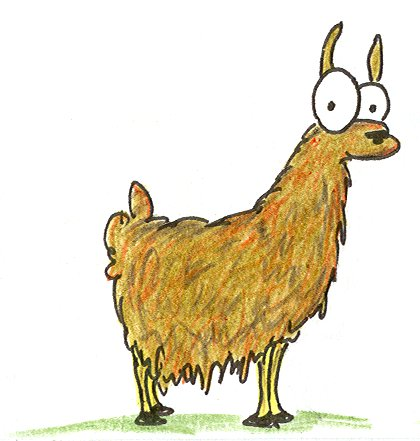
\includegraphics[scale=0.1]{llama.jpg}};}
      \onslide<5->{\node (mcsplit) at (2, 2) {\textsc{Cachet}};}
      \onslide<5->{\node (mcsplitdown) at (4, 2) {\textsc{c2d}};}
      \onslide<5->{\node (clique) at (6, 2) {\textsc{d4}};}
      \onslide<5->{\node (kdown) at (8, 2) {\textsc{miniC2D}};}
      \onslide<5->{\node (kdown2) at (10, 2) {\textsc{DPMC}};}
      \onslide<7->{\node (answer) at (2, 0) {answer};}
      \path[->]<3-> (graphs) edge node[above] {\VarClock} (features);
      \path[->]<4-> (features) edge (ml);
      \only<2-5>{\tikzset{properties/.style={}}}
      \only<6->{\tikzset{properties/.style={ultra thick}}}
      \draw<5->[->] (ml) edge[properties] (mcsplit);
      \draw<5-> [->] (ml) edge (mcsplitdown);
      \path[->]<5-> (ml) edge (clique);
      \path[->]<5-> (ml) edge (kdown);
      \path[->]<5-> (ml) edge (kdown2);
      \path[->]<7-> (mcsplit) edge node[right] {\VarClock} (answer);
      \draw<7->[->] (graphs) edge [bend right=40] (2, 1);
    \end{tikzpicture}
\end{frame}

\begin{frame}[allowframebreaks]
        \frametitle{References}
        \printbibliography
\end{frame}

\end{document}
